\clearpage

\section{Resolució del problema}

\subsection{Dades físiques i numèriques}

La geometria del problema ve donada per
\[
	R_1 = 0.10 \ \si{m} \qquad
	R_2 = 0.10 \ \si{m} \qquad
	H = 1 \ \si{m}
\]
Les propietats termofísiques del cilindre són:
\[
	\dot{q}_v = 10^{4} \ \si{\frac{\watt}{\meter^2}} \qquad
	\rho = 2700 \ \si{\frac{\kilo\gram}{\meter^3}} \qquad
	c_{p} = 900 \ \si{\frac{\joule}{\kilo\gram \, \kelvin}} \qquad
	\lambda = 50 \ \si{\frac{\watt}{\meter \,\kelvin}}	
\]
Les propietats termofísiques dels fluids són les següents:
\[
	\begin{aligned}
		\alpha_A &= 1300 \ \si{\frac{\watt}{\meter^2}} & \qquad
		T_A(t) &= 30 + 20 \, \sin(\frac{2 \pi}{3600} t) \ \si{\celsius} \\
		\alpha_B &= 120 \ \si{\frac{\watt}{\meter^2}} & \qquad
		T_B(t) &= 30 + 5 \, \sin(\frac{2 \pi}{24 \cdot 3600} t) \ \si{\celsius}
	\end{aligned}
\]
Per últim, les dades numèriques són $N = 50$, $\delta = 10^{-6}$, $\beta = \frac{1}{2}$, $\Delta t = 1 \ \si{\second}$ i $T_0^\star = 30 \ \si{\celsius}$.

\subsection{Gràfiques}

\begin{figure}[h]
	\centering
	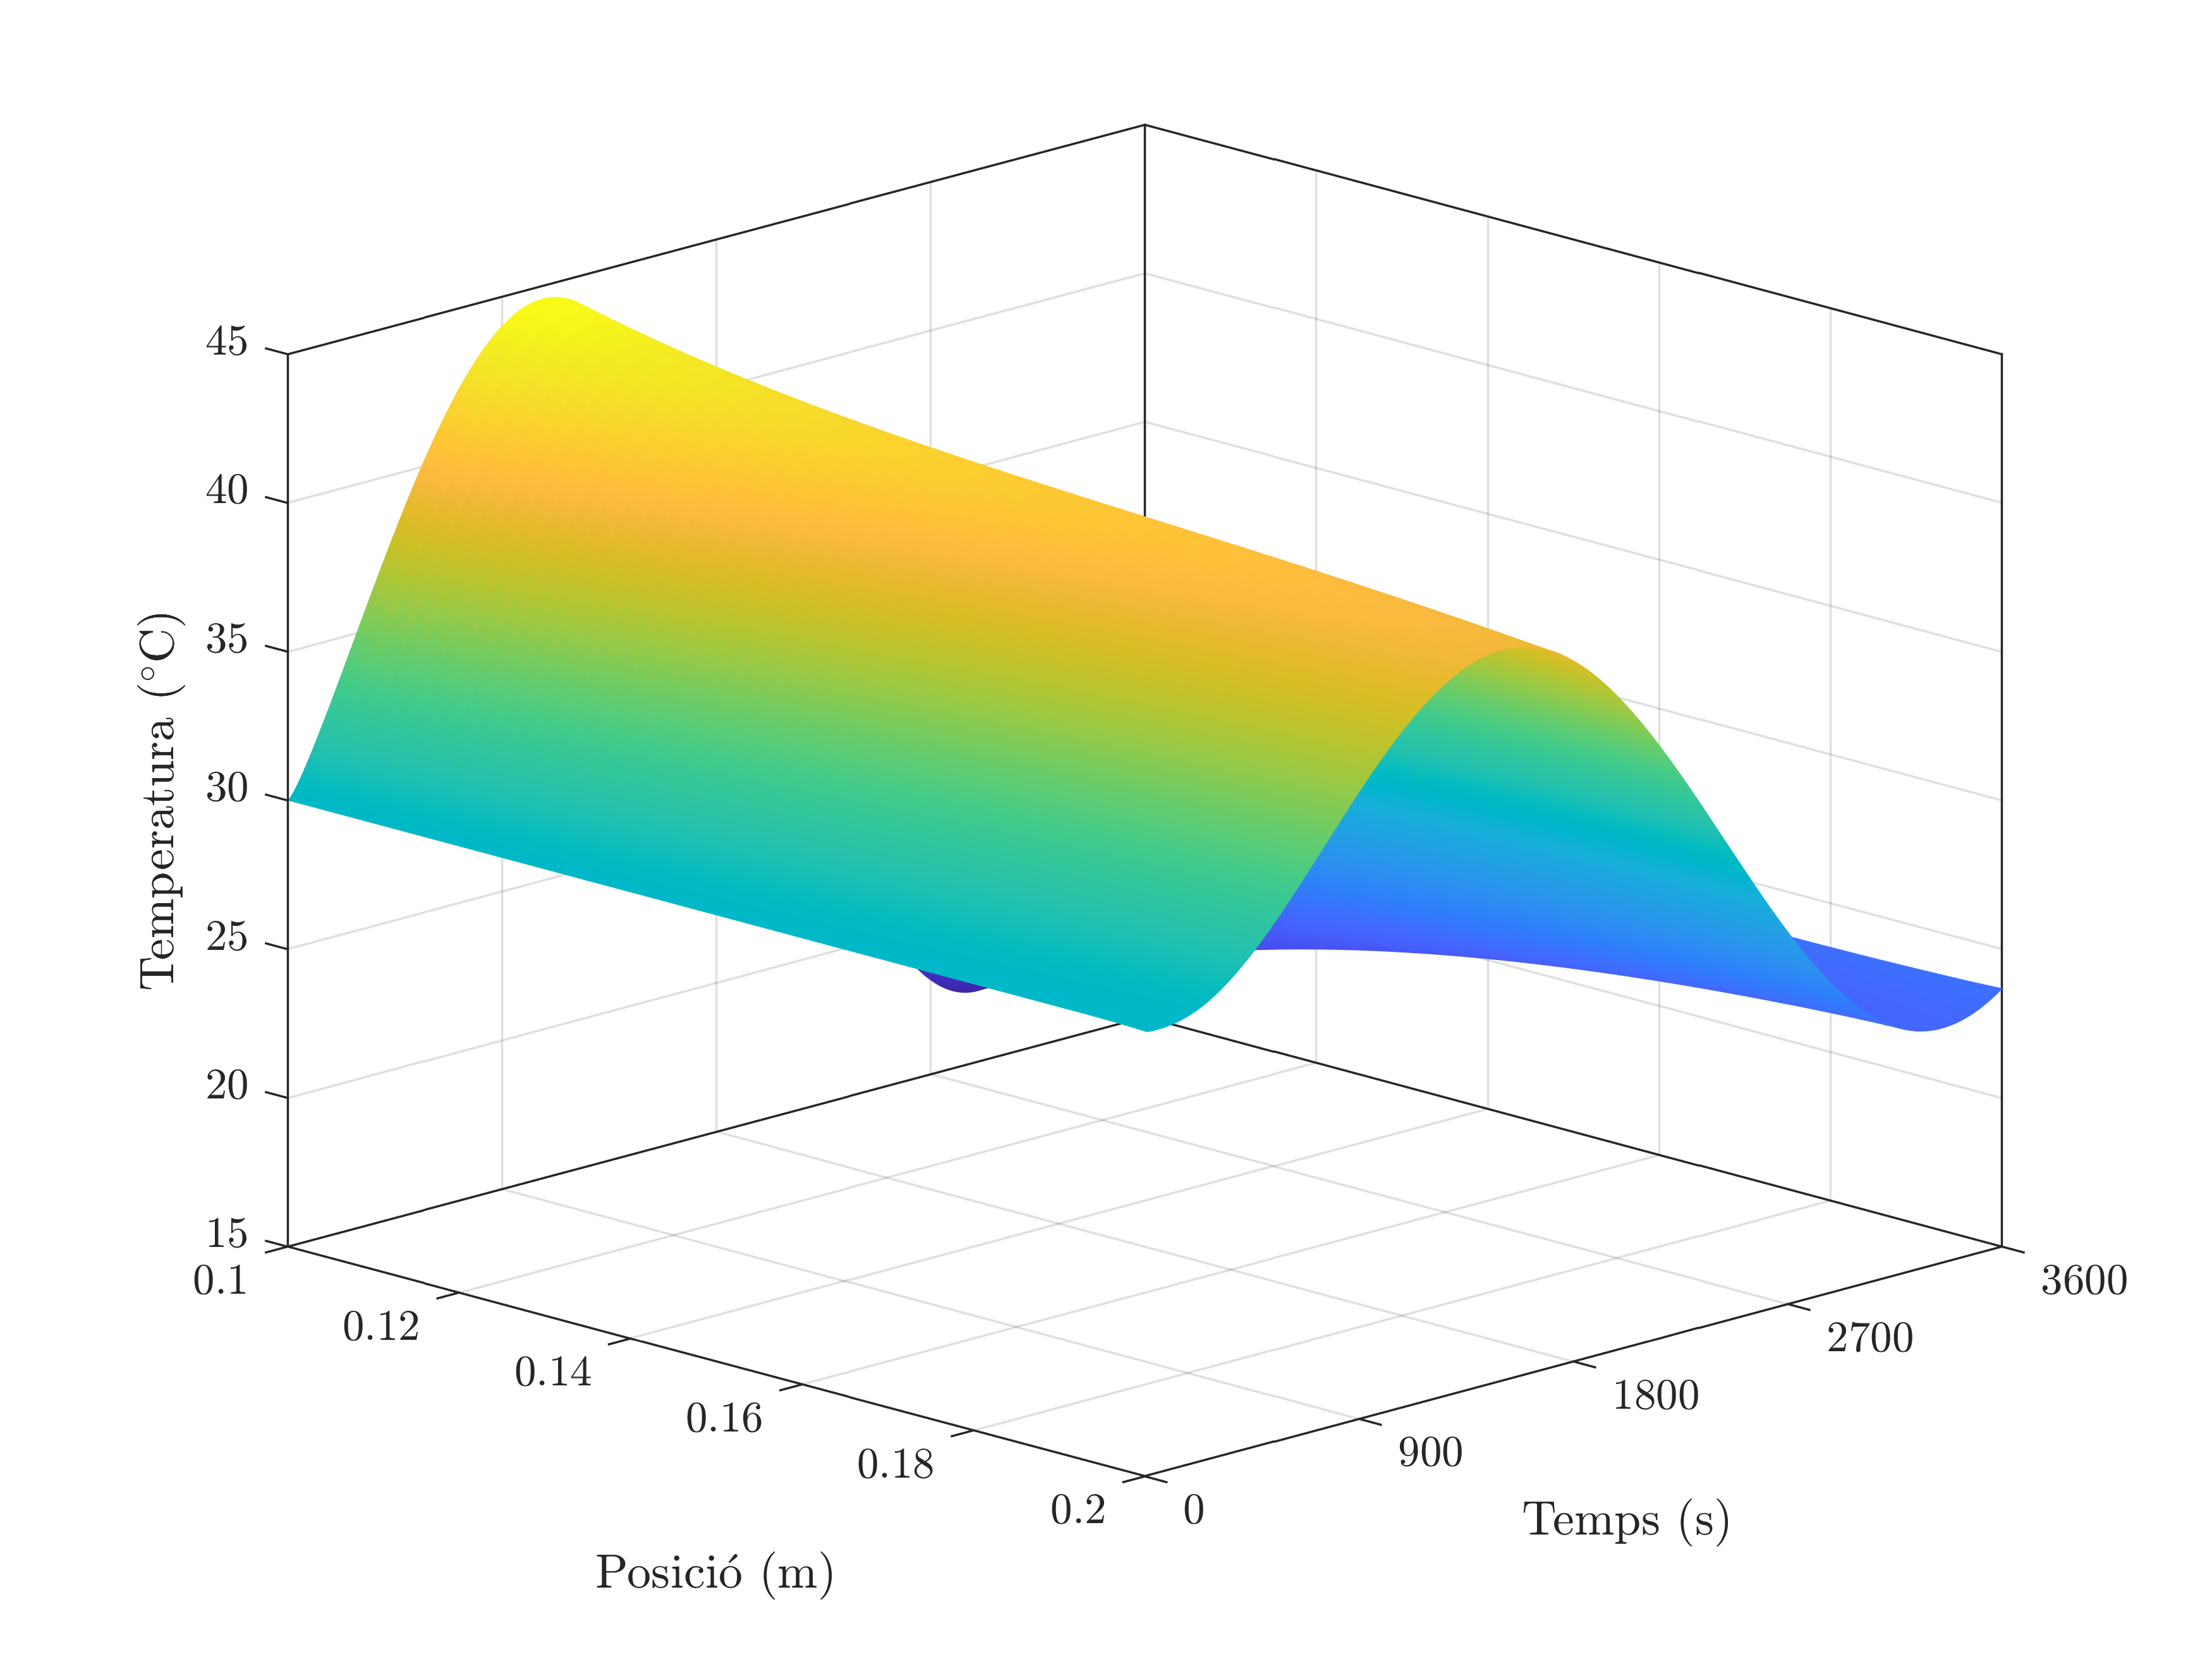
\includegraphics[width=0.8\textwidth]{imagenes/03_resolucio/plot_3d.png}
	\caption{Superfície Temperatura--Posició--Temps}
	\label{fig:plot_3d}
\end{figure}

\begin{figure}[ht]
	\centering
	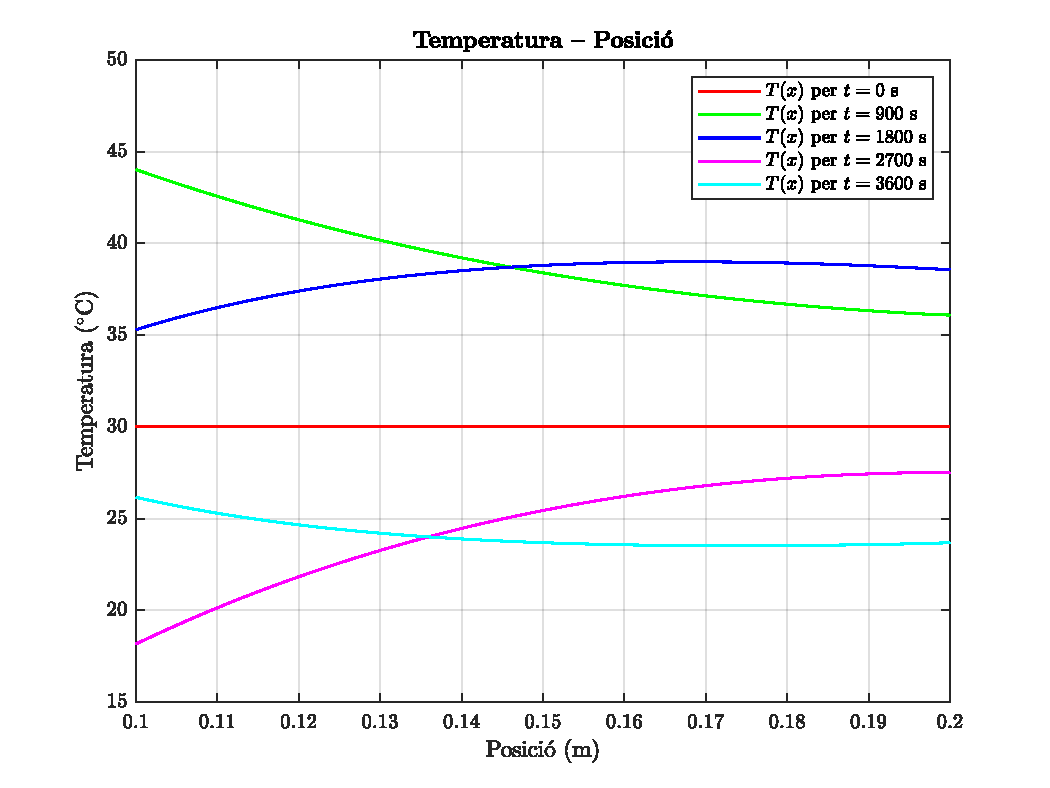
\includegraphics[width=0.8\textwidth]{imagenes/03_resolucio/temperatura_posicio.pdf}
	\captionsetup{width=0.8\textwidth}
	\caption{Temperatura en funció de la posició $(T(x))$ pels temps $0 \ \si{\second}$, $900 \ \si{\second}$, $1800 \ \si{\second}$, $2700 \ \si{\second}$ i $3600 \ \si{\second}$.}
	\label{fig:temperatura_posicio}
\end{figure}

